
\section{Addition and Multiplication}
\label{sec5::subsection::addition-multiplication}
In this section we prove that the addition and multiplication of two \effectivelyOpen{} functions $f,g:\Reals\to\Reals$, defined as $(f+g)(x)=f(x)+g(x)$ and $(f\ldots g)(x)=f(x)\cdot g(x)$ respectively, are \effectivelyOpen{}.
In order to do this, we first break down the addition and multiplication into atomic functions (that when composed together give us our original addition and multiplication) and prove that each of these atomic functions are \effectivelyOpen{}. Then using Theorem \ref{thm::composition_has_OEX}, we can immediately imply that our original addition and multiplication are \effectivelyOpen{}.
\subsection{Deconstruction of Addition and Multiplication}
\label{sec::deconstruction-addition-multiplication}
In order to prove properties about addition ($(f+g)(x) = f(x)+g(x)$) we deconstruct $(f+g)(x)$ into the composition of
    \begin{itemize}
        \item addition: $\Add(x,y) = x + y$,
        \item cartesian product: $\CartProd(x,y) = (f(x),g(y))$, 
        \item diagonal: $\Diag(x) = (x,x)$.
    \end{itemize}
This gives us 
\begin{align*}
    \Add(\CartProd(\Diag(x))) & = (\Add(\CartProd(x,x)))\\
    & = (\Add(f(x),g(x)))\\
    & = f(x)+g(x)
\end{align*}
Similarly, in order to prove properties about multiplication ($(f\cdot g)(x) = f(x)\cdot g(x)$) we deconstruct $(f\cdot g)(x)$ into the composition of
    \begin{itemize}
        \item multiplication: $\Mult(x,y) = x \cdot y$,
        \item cartesian product: $\CartProd(x,y) = (f(x),g(y))$, 
        \item diagonal: $\Diag(x) = (x,x)$.
    \end{itemize}
This gives us 
\begin{align*}
    \Mult(\CartProd(\Diag(x))) & = (\Mult(\CartProd(x,x)))\\
    & = (\Mult(f(x),g(x)))\\
    & =f(x)\cdot g(x)
\end{align*}

\subsection{\EffectiveOpenness{} for addition}
\begin{claim}
    \label{claim::add-effectively-open}
    The function $\Add:\Reals\times\Reals \to \Reals$ with $\Add(x,y) = x + y$ is \effectivelyOpen.
\end{claim}
\begin{proof}
    Using Remark \ref{remark::OEX_for_interval_implies_OEX_for_all_open_sets}, we only need to prove that for any interval $I=(a,b)$ with rational endpoints, we have an effective open exhaustion for $f^{-1}(I)$, i.e.,  
    \[
    \Add^{-1}(I) = \curlybrac{(x,y)\mid x+y \in (a,b)}
    \]
    has an effective open exhaustion. Now using Theorem \ref{thm::rec_in_implies_OEX} we only need to present a recursive function deciding if any arbitrary $2$-cube $(x_1, x_2) \times (y_1, y_2)$ is in $\Add^{-1}[I]$. As shown in Figure \ref{Figure::helper_Add_invers}, we can define 
    \[
    \isIn_{\Add^{-1}(I)}(x_1, y_1, x_2, y_2) \stackrel{def}= a<x_1+y_1< b\quad \land \quad a< x_2+y_2<b.
    \]
    Since $x_1, y_1, x_2, y_2$ are all rational, this function is clearly recursive, and this, along with Theorem \ref{thm::rec_in_implies_OEX}, gives us an effective open exhaustion for $\Add^{-1}(I)$.
    \begin{figure}[!ht]
    \centering
    \caption{Visualization of a 2-cube contained in $\Add^{-1}((a,b))$}
    \label{Figure::helper_Add_invers}
    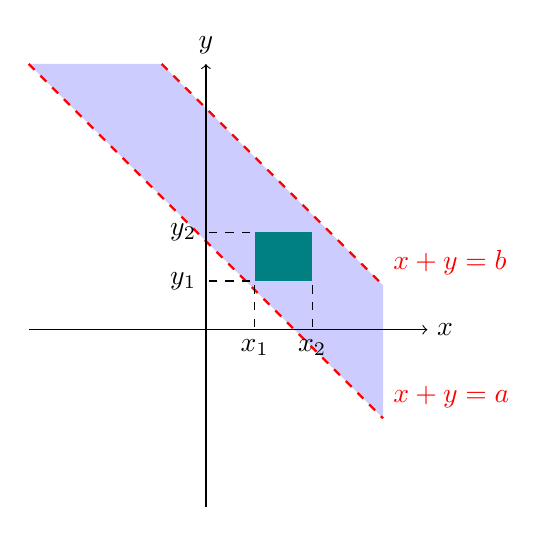
\begin{tikzpicture}[scale=0.75] % Scale everything to 3/4

        % Define parameters
        \def\a{1.5}  % Scaled to 3/4
        \def\b{3.75}  % Scaled to 3/4
        \def\xmin{-3}  % Scaled to 3/4
        \def\xmax{3}  % Scaled to 3/4
        \def\ymin{-3}  % Scaled to 3/4
        \def\ymax{3}  % Scaled to 3/4

        % Shade the region between the two lines
        \fill[blue!20] (\xmin, \a-\xmin) -- (\xmax, \a-\xmax) -- (\xmax, \b-\xmax) -- (-0.75, 4.5) -- cycle;

        % Draw the boundary lines
        \draw[thick, red, dashed] (\xmin, \a-\xmin) -- (\xmax, \a-\xmax) node[anchor=south west] {$x+y=a$};
        \draw[thick, red, dashed] (-0.75, 4.5) -- (\xmax, \b-\xmax) node[anchor=south west] {$x+y=b$};

        % Axes
        \draw[->] (\xmin, 0) -- (\xmax+0.75, 0) node[right] {$x$};
        \draw[->] (0, \ymin) -- (0, \ymax+1.5) node[above] {$y$};

        % square
        \fill[teal] (0.825, 0.825) rectangle (1.8, 1.65);

        % labels
        \draw[thin, black, dashed] (0.75, 0.825) -- (0, 0.825) node[left] {$y_1$};
        \draw[thin, black, dashed] (1.8, 0.75) -- (1.8, 0) node[below] {$x_2$};
        \draw[thin, black, dashed] (0.75, 1.65) -- (0, 1.65) node[left] {$y_2$};
        \draw[thin, black, dashed] (0.825, 0.75) -- (0.825, 0) node[below] {$x_1$};

    \end{tikzpicture}
\end{figure}

   
\end{proof}

\begin{claim}
    \label{claim::cartprod-effectively-open}
    Let $f,g:\Reals\to\Reals$ be effectively open. Then, the function $\CartProd:\Reals\times\Reals \to \Reals\times\Reals$ with $\CartProd(x,y) = (f(x), g(y))$ is \effectivelyOpen.
\end{claim}
\begin{proof}
    In order to prove this, we need to prove that for any open $U\subseteq \Reals\times\Reals$ with an open exhaustion, the set 
    \[
    \CartProd^{-1}(U) = \curlybrac{(x,y)\mid (f(x), g(y)) \in U}
    \]
    has an effective open exhaustion. It suffices to prove that for each $2$-cube $I_1\times I_2$, 
    \[
    (f\times g)^{-1}(I_1\times I_2)\ = \curlybrac{(x,y) \mid (f(x), g(x)) \in I_1\times I_2}
    \]
    has an effective open exhaustion. We have
    \[
        (f\times g)^{-1}(I_1\times I_2)
        \BLOCK{
        =\curlybrac{(x,y) \mid (f(x), g(x)) \in I_1\times I_2}\\
        =\curlybrac{(x,y) \mid f(x) \in I_1 \land g(x) \in I_2}\\
        =\curlybrac{(x,y) \mid f(x) \in I_1} \ \cap\ \curlybrac{(x,y) \mid g(x) \in I_2}\\
        =f^{-1}(I_1) \times \Reals\ \cap\ \Reals\times g^{-1}(I_2)\\
        =f^{-1}(I_1) \times g^{-1}(I_2)
        }
    \]
    Since $f,g$ are \effectivelyOpen, and $I_1, I_2$ are open finite intervals and hence have open exhaustions, $f^{-1}(I_1)$ and $g^{-1}(I_2)$ both have open exhaustions respectively $(F_0, F_1, \ldots)$ and $(G_0, G_1, \ldots)$. Then 
    $(F_0 \times G_0, F_1 \times G_1, \ldots)$ is an effective open exhaustion for $f^{-1}(I_1) \times g^{-1}(I_2)$.
    
\end{proof}
% \begin{proof}
%     Using Remark \ref{remark::OEX_for_interval_implies_OEX_for_all_open_sets-r2}, we only need to prove that for any interval $I=(a,b)$ with rational endpoints, we have an effective open exhaustion for $f^{-1}(I)$, i.e.,  
%     \[
%     \Add^{-1}[I] = \curlybrac{(x,y)\mid x+y \in (a,b)}
%     \]
%     has an effective open exhaustion. Now using Theorem \ref{} we only need to present a recursive function deciding if $\nbox_N(a_1, a_2)$ is in $\Add^{-1}[I]$. We define 
%     \[
%     \isIn_{\Add^{-1}[I]}(N, a_1, a_2) \stackrel{def}= a<a_1/{2^{N}}+a_2/{2^{N}}< b\quad \land \quad a< {a_1+ a_2+2}/{2^{N}}<b.
%     \]
% \end{proof}
\begin{claim}
    \label{claim::diag-effectively-open}
    The function $\Diag:\Reals\to \Reals\times\Reals$ with $\Diag(x) = (x,x)$ is \effectivelyOpen.
\end{claim}
\begin{proof}
    In order to prove this, we need to prove that for any open $U\subseteq \Reals\times\Reals$ with an effective open exhaustion, the set 
    \[
    \Diag^{-1}(U) = \curlybrac{x\mid (x,x) \in U}
    \]
    has an effective open exhaustion.
    We give an algorithm that outputs each stage of an effective open exhaustion for $\Diag^{-1}(U)$.
    For any $l\in \Nats$ of the given effective open exhaustion for $U$, the stage $U_l$ consists of open $2$-cubes 
    \[
    (x_1^l, x_2^l)\times (y_1^l, y_2^l), \ldots, (x_{2k_l-1}^l, x_{2k_l}^l)\times (y_{2k_l-1}^l, y_{2k_l}^l).
    \]
    For any $2$-cubes $(x_i^l, x_{i+1}^l)\times (y_i^l, y_{i+1}^l)$ 
    we can construct an open interval
    \[
    I_i^l \stackrel{def}= (x_i^l, x_{i+1}^l)\cap(y_i^l, y_{i+1}^l),
    \]
    as shown\footnote{In this figure, the superscript $l$ for endpoints of each interval is removed since we are only concerned with the $l$th stage at this point.} in Figure \ref{Figure::helper_Diag_invers}, and we can define $U_l \stackrel{def}= I_1^l, \ldots, I_{k_l}^l$. Then the sequence $(U_1, U_2, \ldots)$ is an open exhaustion for $\Diag^{-1}(U)$. 
    \begin{figure}[!ht]
    \centering
    \caption{Visualization of a 2-cube contained in $\Diag^{-1}(U)$}
    \label{Figure::helper_Diag_invers}
    \begin{tikzpicture}
        % Define parameters
        \def\a{2}
        \def\b{5}
        \def\xmin{-1}
        \def\xmax{4}
        \def\ymin{-1}
        \def\ymax{4}
        
        % square
        \fill[blue!20] (1, 2) rectangle (5, 3);
        \draw[thick, blue, dashed] (1, 2) rectangle (5, 3);

        % rotated
        \fill[red!20] (2, 1) rectangle (3, 5);
        \draw[thick, red, dashed] (2, 1) rectangle (3, 5);

        % intersection
        \fill[pattern=north west lines, pattern color=violet] (2, 2) rectangle (3, 3);
        \draw[violet, thick, dashed] (2, 2) rectangle (3, 3);

        % labels

        \draw[thick, gray, dashed] (3, 1) -- (3, 0) node[below] {$y_{i+1}$};
        \draw[thick, gray, dashed] (2, 1) -- (2, 0) node[below]
        {$y_i$};

        \draw[thick, blue, dashed] (1, 2) -- (1, 0) node[below] {$x_i$};
        \draw[thick, gray, dashed] (3, 5) -- (0, 5) node[left] {$x_{i+1}$};
        \draw[thick, blue, dashed] (5, 3) -- (5, 0) node[below] {$x_{i+1}$};
        
        \draw[thick, blue, dashed] (1, 2) -- (0, 2) node[left] {$y_i$};
        \draw[thick, blue, dashed] (1, 3) -- (0, 3) node[left] {$y_{i+1}$};

        
        \draw[thick, gray, dashed] (2, 1) -- (0, 1) node[left] {$x_i$};


        % Axes
        \draw[->] (\xmin, 0) -- (\xmax+2, 0) node[right] {$x$};
        \draw[->] (0, \ymin) -- (0, \ymax+2) node[above] {$y$};
        \draw (\ymin, \ymin) -- (\xmax+1.5, \ymax+1.5) node[above] {$x = y$};

        \draw[->, purple] (5, 3.5) .. controls (4.4,4.4) .. (3.5, 5);
        
        
        
    \end{tikzpicture}
\end{figure}
\end{proof}

\begin{theorem}[Addition]
\label{thm::addition_has_OEX}
    Let $f,g:\Reals\to \Reals$ be \effectivelyOpen. Then $(f+g)$ is also \effectivelyOpen.
\end{theorem}
\begin{proof}
    Using Theorem \ref{thm::composition_has_OEX}, we know that compositions preserve \effectivelyOpen\text{ness}. Now we know that $(f+g)$ is composed from the functions $\Add$, $\CartProd$, and  $\Diag$. Therefore Lemmas \ref{claim::add-effectively-open}, \ref{claim::cartprod-effectively-open}, and \ref{claim::diag-effectively-open} complete the proof.
\end{proof}

\subsection{\EffectiveOpenness{} for multiplication}
\begin{claim}
\label{claim::mult-effectively-open}
    The function $\Mult:\Reals\times\Reals \to \Reals$ with $\Mult(x,y) = x \cdot y$ is \effectivelyOpen.
\end{claim}
\begin{proof}
    In order to prove this, we need to prove that for any open $U\subseteq \Reals$, the set 
    \[
    \Mult^{-1}(U) = \curlybrac{(x,y)\mid x\cdot y \in U}
    \]
    has an effective open exhaustion. Now using Theorem \ref{thm::rec_in_implies_OEX} we only need to present a recursive function deciding if any arbitrary $2$-cube $(x_1, x_2) \times (y_1, y_2)$ is in $\Mult^{-1}[I]$. Since $x\cdot y$ is a continuous function over the rectangle, its maximum value occurs at one of the corners. This means we can define 
    \begin{align*}
    \isIn_{\Mult^{-1}(I)}(x_1, y_1, x_2, y_2) \stackrel{def}= &
    a<x_1\cdot y_1< b\ \land \ a< x_1\cdot y_2<b\ \land \\
    & a<x_2\cdot y_1<b \ \land\ a<x_2\cdot y_2<b.
    \end{align*}
    Since $x_1, y_1, x_2, y_2$ are all rational, this function is clearly recursive and this, along with Theorem \ref{thm::rec_in_implies_OEX}, gives us an effective open exhaustion for $\Mult^{-1}(I)$.
    % \begin{figure}[H]
    \centering
    \caption{Visualization of a 2-cube contained in $\Mult^{-1}(I) = (a,b)$}
    \label{Figure::helper_Mult_invers}
    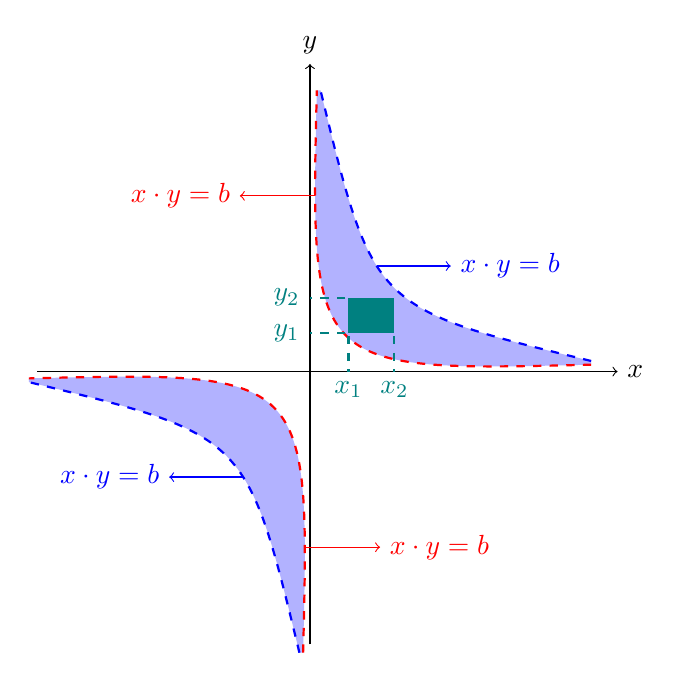
\begin{tikzpicture}[scale=0.67] % Scale everything to 2/3
    
        % Define parameters
        \def\a{1.33}  % Scaled to 2/3
        \def\b{3.33}  % Scaled to 2/3
        \def\xmin{-2.67}  % Scaled to 2/3
        \def\xmax{3.33}  % Scaled to 2/3
        \def\ymin{-2.67}  % Scaled to 2/3
        \def\ymax{3.33}  % Scaled to 2/3

        \fill[blue!30] 
        (\xmax+2, 0.13) .. controls (0,0) .. (0.13, \ymax+2)
        -- 
        (0.2, \ymax+2) .. controls (1.2,1.2) .. (\xmax+2, 0.2)
        -- cycle;

        % negative part
        \fill[blue!30] 
        (-0.13, -\xmax-2) .. controls (0,0) .. (-\ymax-2, -0.13)
        -- 
        (-\ymax-2, -0.2) .. controls (-1.2,-1.2) .. (-0.2, -\xmax-2)
        -- cycle;

        % positive part
        \draw[thick, red, dashed] (\xmax+2, 0.13) ..controls (0,0) .. (0.13, \ymax+2);
        \draw[thick, blue, dashed] (\xmax+2, 0.2) ..controls (1.2,1.2) .. (0.2, \ymax+2);
        
        % Reflected lines
        \draw[thick, red, dashed] (-0.13, -\xmax-2) .. controls (0,0) .. (-\ymax-2, -0.13);
        \draw[thick, blue, dashed] (-0.2, -\xmax-2) .. controls (-1.2,-1.2) .. (-\ymax-2, -0.2);

        % Axes
        \draw[->] (\xmin-2.5, 0) -- (\xmax+2.5, 0) node[right] {$x$};
        \draw[->] (0, \ymin-2.5) -- (0, \ymax+2.5) node[above] {$y$};

        % square
        \fill[teal] (0.73, 0.73) rectangle (1.6, 1.4);

        % labels
        \draw[thick, teal, dashed] (0.67,0.73) -- (0,0.73) node[left] {$y_1$};
        \draw[thick, teal, dashed] (1.6,0.67) -- (1.6,0) node[below] {$x_2$};
        \draw[thick, teal, dashed] (0.67,1.4) -- (0,1.4) node[left] {$y_2$};
        \draw[thick, teal, dashed] (0.73,0.67) -- (0.73,0) node[below] {$x_1$};

        % labels
        \draw[blue, ->] (1.27, 2) -- (2.67, 2) node[right] {$x \cdot y = b$};
        \draw[blue, ->] (-1.27, -2) -- (-2.67, -2) node[left] {$x \cdot y = b$};
        \draw[red, ->] (0.1, 3.33) -- (-1.33, 3.33) node[left] {$x \cdot y = b$};
        \draw[red, ->] (-0.1, -3.33) -- (1.33, -3.33) node[right] {$x \cdot y = b$};
        
    \end{tikzpicture}
\end{figure}


\end{proof}
\begin{theorem}[Multiplication]
\label{thm::multiplication_has_OEX}
     Let $f,g:\Reals\to \Reals$ be \effectivelyOpen. Then $(f\cdot g)$ is also \effectivelyOpen.
\end{theorem}
\begin{proof}
       Using Theorem \ref{thm::composition_has_OEX}, we know that compositions preserve \effectivelyOpen\text{ness}. Now we know that $(f\cdot g)$ is composed from the functions $\CartProd$, $\Diag$, and $\Mult$. Therefore Lemmas \ref{claim::cartprod-effectively-open}, \ref{claim::diag-effectively-open}, and \ref{claim::mult-effectively-open} complete the proof.
\end{proof}
